\section{Fondamenti teorici}
\subsection{Il problema difficile della coscienza}
Chalmers (1995) formulò il problema difficile così: nessuna combinazione di grandezze fisiche, per quanto complessa, implica logicamente l'esistenza di esperienza soggettiva. Tutte le descrizioni fisiche --- neurali, computazionali, funzionali --- descrivono ciò che il cervello fa. Non descrivono come sia essere un cervello. Non descrivono perché l'esperienza esista. Ciò che propongo: la coscienza non è generata dal cervello. Il cervello è un ricevitore. L'esperienza è la trasduzione del campo akashico.

\subsection{Il monismo russelliano}
Russell (1927) osservò qualcosa di profondo: la fisica descrive le proprietà strutturali della materia --- massa, carica, spin, posizione --- ma tace completamente sulla natura intrinseca di ciò che porta queste proprietà. Sia S un sistema fisico qualsiasi: R(S) indica le sue proprietà relazionali/strutturali e I(S) le sue proprietà intrinseche. La tesi russelliana afferma che I(S) è proto-esperienziale per ogni S.

\subsection{Integrated Information Theory}
Tononi (2004, 2008) offre un quadro matematico per quantificare la coscienza:
\begin{equation}
\Phi = \min_{\{P \in P\}} D_{KL}(p(X_{t+1})|X_{t}) \parallel \prod_{i} p(x_{i} \land (t+1)|x_{i} \land t))
\end{equation}
Spiegazione semplice: $\Phi$ misura quanto è integrata l'informazione in un sistema. Più $\Phi$ è grande, più ricca è l'esperienza del sistema.

\subsection{Orchestrated Objective Reduction}
Penrose (1996) propone che le sovrapposizioni quantistiche subiscano un collasso gravitazionale spontaneo quando l'energia di sovrapposizione $E_G$ raggiunge una soglia:
\begin{equation}
\tau \approx \frac{\hbar}{E_G}
\end{equation}
Ciò che mi ha interessato: la frequenza di collasso per i microtubuli corticali è $\tau \approx 25$ ms, che corrisponde a $\sim 40$ Hz --- esattamente la frequenza delle oscillazioni gamma, il marcatore empirico più robusto degli stati coscienti. Supporto sperimentale: Babcock et al. (2024) hanno mostrato superradianza ultravioletta nei microtubuli a temperatura ambiente; Kalra et al. (2023) hanno mostrato che i gas anestetici attenuano specificamente gli effetti ottici quantistici nei microtubuli.

\subsection{Kaluza--Klein e teoria F}
Theodor Kaluza propose nel 1919 l'unificazione della gravitazione con l'elettromagnetismo mediante una quinta dimensione. Einstein ne fu entusiasta e lavorò a questa teoria tra il 1938 e il 1943. La formulazione originale:
\begin{equation}
dS^2 = g_{\mu\nu} dx^\mu dx^\nu + \varphi^2(dx^5 + A_{\mu} dx^\mu)^2
\end{equation}

\subsection{Il campo Akasha}
Il concetto di Akasha (sanscrito: \emph{ākāśa}) è un elemento fondamentale della filosofia indiana. Akasha è l'elemento più sottile, immateriale. È il primo che si è manifestato nell'universo. Da esso si sarebbero sviluppati tutti gli altri elementi. Nella teosofia, Akasha è reinterpretato come un campo informazionale universale (Laszlo, 2014). Gli «archivi akashici» registrano tutti gli eventi dell'universo. L'ipotesi ART-12D: Akasha è il campo quantistico della materia oscura. \textit{Nota: Akasha è usato qui solo come metafora di un campo fisico, non come entità religiosa.}

\subsection{Materia grigia vs materia oscura}
La materia grigia è il tessuto del sistema nervoso centrale composto principalmente da corpi cellulari neuronali, dendriti, terminali assonici non mielinizzati e cellule gliali. È la sede dell'elaborazione dell'informazione. La materia bianca è composta da assoni mielinizzati ed è responsabile della trasmissione.

\subsection{Una definizione operativa della coscienza}
Propongo una definizione operativa che separa il contenuto della coscienza dalla capacità di integrarlo:
\begin{equation}
C_{\text{total}} = I_{\text{content}} \times C_{\text{awareness}}
\end{equation}
dove $I_{\text{content}}$ è l'informazione strutturata (il contenuto dell'esperienza) e $C_{\text{awareness}}$ è la consapevolezza (la capacità di sapere di sapere). Pensi a una macchina fotografica. Cattura immagini (informazione), ma non sa di catturarle. Una persona con una macchina fotografica cattura immagini E sa di catturarle. Allo stesso modo, la coscienza è informazione + consapevolezza.

\subsection{La convergenza con Dulcan}
Dumitru Constantin Dulcan (n. 1938), neurologo e psichiatra, pubblicò nel 1981 «L'intelligenza della materia», insignito nel 1992 del premio di filosofia «Vasile Conta» dell'Accademia Rumena. Le idee che mi hanno influenzato: la coscienza non è generata dal cervello ma lo usa come strumento; il subconscio contiene l'intelligenza infinita dell'Universo; il pensiero è la forza più potente dell'universo, con una frequenza e un campo energetico propri; esiste un campo di energia e luce che coordina la materia. La convergenza con ART-12D: Dulcan fornisce l'intuizione concettuale, ART-12D fornisce la formalizzazione matematica e le predizioni testabili.

\subsection{La struttura tripartita dell'entità umana}
Propongo un modello tripartito dell'entità umana, analogo agli stati di aggregazione dell'acqua:
\begin{table}[H]
\centering
\begin{tabular}{@{}llll@{}}
\toprule
\textbf{Stato} & \textbf{Entità umana} & \textbf{Substrato} & \textbf{Corrispondenza ART-12D} \\ \midrule
Solido & Corpo fisico & Materia & M (materia ordinaria) \\
Liquido & Anima & Energia & E (il campo della coscienza) \\
Gassoso & Spirito & Informazione & Sp (il campo akashico) \\ \bottomrule
\end{tabular}
\end{table}
Formalizzazione: $H = M + E + Sp$. Conseguenze: la morte non distrugge l'entità, cambia solo lo stato dominante; la coscienza può accedere a ciascuno dei tre stati; la malattia compare quando uno degli stati è squilibrato.

\subsection{Le forme del pensiero come strutture informazionali}
I pensieri non sono solo attività neuronale, ma strutture informazionali che possono assumere forme molteplici. Immaginato (visualizzazione interna, il campo della coscienza), pronunciato (la parola parlata, il campo akashico + un'onda sonora), scritto (testo scritto, materia + informazione), disegnato (rappresentazione visiva, materia + forma). Formalizzazione generale: $F_{\text{thought}} = \sum_{\text{forms}} \alpha_i F_i$.

\subsection{L'empatia come risonanza di frequenza}
L'empatia può essere formalizzata come caso particolare della telepatia, in cui l'accoppiamento è emotivo e non informazionale. Formalizzazione:
\begin{equation}
\text{Empathy}(A,B) = \frac{1}{1 + \frac{(\omega_A - \omega_B)^2}{\Gamma^2}}
\end{equation}
Interpretazione: quando le frequenze coincidono ($\omega_A = \omega_B$), l'empatia è massima; quando differiscono, l'empatia diminuisce; l'empatia non dipende dalla distanza (il campo è onnipresente). Predizione testabile: le coppie con empatia elevata dovrebbero mostrare correlazioni EEG più forti delle coppie con empatia bassa.

\subsection{La parola come eccitazione del campo akashico}
Propongo che la materia oscura abbia una manifestazione acustica --- uno spettro di oscillazioni che possono essere eccitate da onde sonore. La motivazione cosmologica: le oscillazioni acustiche primordiali (BAO) sono fluttuazioni della densità di materia che si sono propagate come onde sonore nell'universo primordiale. In ART-12D, queste oscillazioni sono oscillazioni del campo akashico. Formalizzazione:
\begin{equation}
A(x,t) = \sum_n A_n \cos(\omega_n t + \varphi_n)
\end{equation}
Lo spettro acustico:
\begin{equation}
\omega_n = \frac{1}{R} \sqrt{n^2 + \mu_A^2 R^2}
\end{equation}
L'accoppiamento parola--campo:
\begin{equation}
L_{\text{int}} = g_{\text{sound}} A \cdot \Phi_{\text{sound}}
\end{equation}
Effetti differenziati: Amore (200-400 Hz, attiva le zone emotive positive), Paura (500-800 Hz, attiva l'amigdala), Guarigione (300-500 Hz, attiva l'attesa positiva), Morte (150-300 Hz, attiva le zone di ansia).

\textbf{Il problema di scala.} Lo spettro acustico $\omega_n$ è fissato dallo stesso raggio di compattificazione che dà la massa alla materia oscura. Per $1/R = 10^{-5}$ eV i modi stanno nella gamma dei GHz, non a qualche centinaio di Hz. Una risonanza a 150--800 Hz richiederebbe $1/R \approx 1,24\times10^{-12}$ eV, circa sette ordini di grandezza sotto la scala di massa. Finché non viene introdotta una seconda scala di compattificazione, la predizione non ha contenuto numerico: l'accoppiamento $g_{\text{sound}}$ non è fissato in modo indipendente.

\begin{figure}[H]
\centering
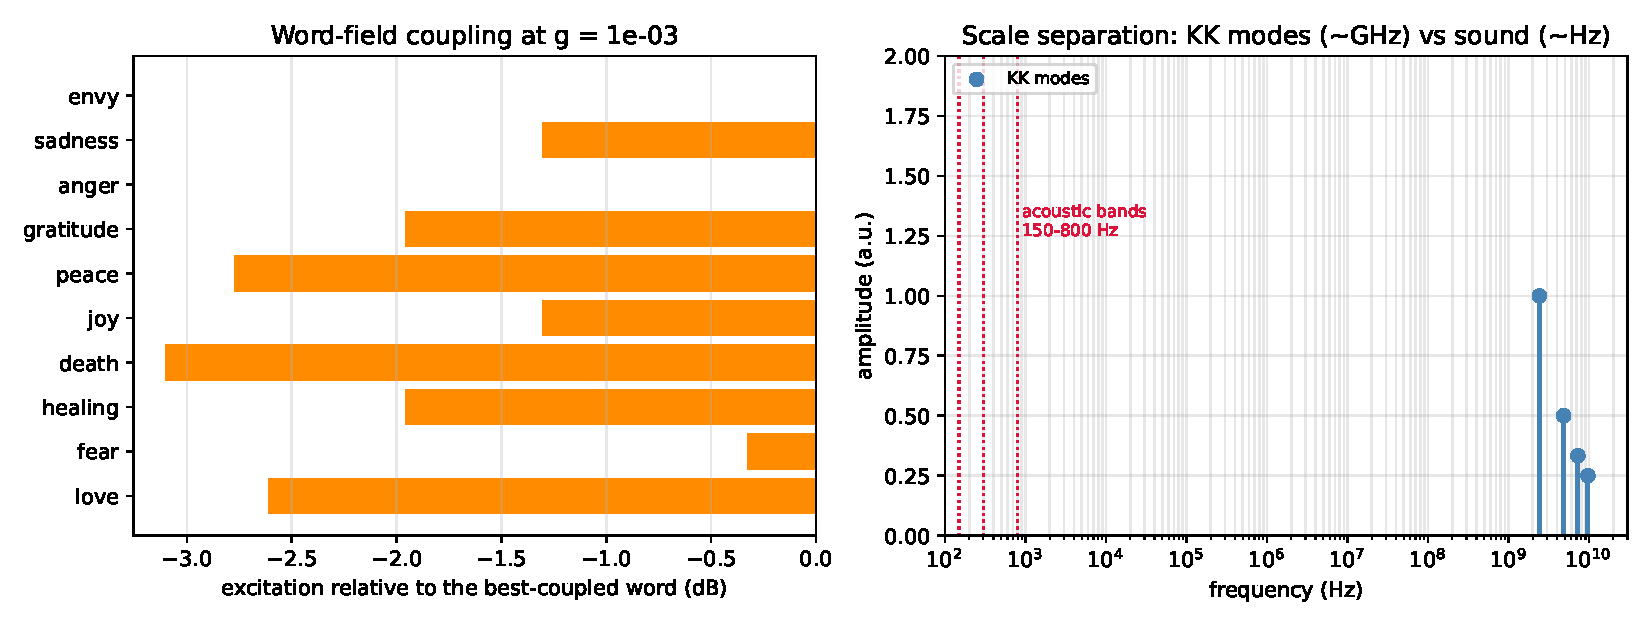
\includegraphics[width=0.9\textwidth]{figures/fig06_word_excitation.pdf}
\caption{A sinistra: l'accoppiamento relativo parola--campo per le dieci bande usate nell'articolo. A destra: la separazione di scala tra i modi KK (~GHz) e le bande acustiche (~Hz).}
\label{fig:cuvant}
\end{figure}

\subsection{Il tempo come vibrazione}
La definizione del secondo: «Un secondo è la durata di 9.192.631.770 periodi della radiazione dell'atomo di cesio-133». Che cosa accade se la frequenza cambia: se la frequenza aumenta, il tempo si comprime; se diminuisce, il tempo si dilata. La risonanza di Schumann: storicamente $\sim 7,83$ Hz, recentemente $\sim 12$ Hz. Il cuore come orologio biologico: paura ($\sim 120$ bpm) --- il tempo vola; meditazione ($\sim 50$ bpm) --- il tempo è dilatato; sonno profondo ($\sim 40$ bpm) --- il tempo scompare. Riferimenti relativi, non assoluti: il cesio (9.192.631.770 Hz), Schumann (7,83--12 Hz), il cuore (1,2 Hz). Tutti sono relativi. Nessuno è «quello vero».
\begin{equation}
\text{Reality} = \frac{\text{Change}}{\text{Reference}}
\end{equation}

\subsection{Realtà multiple e multiverso}
Il campo akashico totale: $A_{\text{total}} = \sum_{k=1}^{N_{\text{vacua}}} A_k$. Lo stato del multiverso: $|\Psi_{\text{multiverse}}\rangle = \otimes_{k=1}^{N_{\text{vacua}}} |A_k\rangle$. L'intersezione delle realtà: le realtà non sono solo parallele --- possono intersecarsi.

\subsection{La biblioteca universale (Akasha)}
Il contenuto del campo: il campo akashico contiene tutta l'informazione --- tutto ciò che è stato, tutto ciò che è, tutto ciò che sarà.
\begin{equation}
A_{\text{total}} = \sum_{\text{(all events)}} A_i
\end{equation}
L'accesso all'informazione:
\begin{equation}
I_{\text{access}}(t) = \int_0^\infty S_A(\omega) S_G(\omega, t) d\omega
\end{equation}
L'indicizzazione: l'informazione è indicizzata per rilevanza, non per tempo.
\begin{equation}
\text{Information received} = \text{Akashic field} \times \text{Relevance}(t)
\end{equation}

\subsection{La gerarchia della ricezione}
\begin{table}[H]
\centering
\begin{tabular}{@{}clcc@{}}
\toprule
\textbf{Livello} & \textbf{Sistema} & \textbf{$\Phi$} & \textbf{Accesso} \\ \midrule
0 & Termostato & 0 & Nessuno \\
1 & C. elegans & Minimo & Chemiotassi \\
2 & Insetto & Basso & Sensazione \\
3 & Topo & Moderato & Emozione \\
4 & Cane & Alto & Empatia \\
5 & Corvide & Alto & Pianificazione \\
6 & Octopode & Distribuito & Risoluzione \\
7 & Umano & Molto alto & Autoriferimento \\
8 & Umano addestrato & Esteso & Metacognizione \\ \bottomrule
\end{tabular}
\end{table}
Il limite della ricezione: $\lim_{\Phi \rightarrow \infty} E(\Phi) = I_{\text{total}}$.

\subsection{La parola come origine: la convergenza delle religioni}
Tutte le grandi tradizioni religiose descrivono la Parola come origine dell'universo. Il cristianesimo ha il Logos --- la Parola (il modo fondamentale del campo). L'induismo ha Om (la vibrazione primordiale). L'islam ha Kun («Sii!»).

\subsection{La manifestazione acustica del campo akashico}
$A(x,t) = \sum_n A_n \cos(\omega_n t + \varphi_n)$. Lo spettro acustico: $\omega_n = \frac{1}{R} \sqrt{n^2 + \mu_A^2 R^2}$.

\subsection{Dio in ART-12D}
Ci sono quattro ipotesi. Dio è il campo akashico stesso. Dio è la fonte del campo. Dio è la coscienza universale. Dio è una proiezione umana. Non so quale sia corretta. Ma la domanda è legittima.

\subsection{Materia oscura ed energia oscura: due facce dello stesso campo}
L'ipotesi ART-12D: la materia oscura e l'energia oscura sono due aspetti dello stesso campo akashico. Formalizzazione:
\begin{equation}
L_A = \frac{1}{2} g^{MN} \partial_M A^* \partial_N A + \frac{1}{2} \mu_A^2 |A|^2 - \frac{\lambda_A}{4} |A|^4
\end{equation}
L'equazione di stato: $w = p_A / \rho_A$. Per un campo oscillante la media temporale si calcola esattamente sull'orbita e dipende dal rapporto $\delta = A_{\text{osc}}/A_{\min}$ tra l'ampiezza di oscillazione e il valore del potenziale nel minimo. Esistono tre regimi distinti:
\begin{center}
\begin{tabular}{@{}lll@{}}
\toprule
\textbf{Regime} & \textbf{Condizione} & $w$ \\ \midrule
Piccola oscillazione attorno al minimo & $\delta \ll 1$ & $0$ (materia) \\
Oscillazione dominata dal termine quartico & $\delta \gg 1$ & $1/3$ (radiazione) \\
Campo congelato al minimo & $\delta = 0$ & $-1$ (costante cosmologica) \\ \bottomrule
\end{tabular}
\end{center}
La versione 30 affermava che il regime di grande ampiezza dà $w \simeq 1$. Il valore corretto è $1/3$: il teorema del viriale dà $\langle K \rangle = 2\langle V \rangle$ per un potenziale dominato dal termine quartico. Il valore $w = 1$ corrisponde a una dominanza cinetica (kination), che le oscillazioni quartiche non raggiungono, mentre $w = -1$ corrisponde al campo congelato, non a una piccola ampiezza.
